
\documentclass[11pt,a4paper]{article}

% ============================================
% PAGE AND FONT FORMATTING
% ============================================

\usepackage[T1]{fontenc}
\usepackage[margin=1in]{geometry}
\usepackage{lmodern}
\usepackage{microtype}
\usepackage{setspace}

% ============================================
% MATHEMATICS
% ============================================

\usepackage{amsmath}
\usepackage{amssymb}

% ============================================
% FIGURES AND TABLES
% ============================================

\usepackage{graphicx}
\usepackage{booktabs}
\usepackage{float}
\usepackage{placeins}

\graphicspath{
    {figures/}
    {../results/figures/}
}

\setlength{\textfloatsep}{9pt plus 2pt minus 2pt}
\setlength{\intextsep}{9pt plus 2pt minus 2pt}
\setlength{\floatsep}{7pt plus 2pt minus 2pt}

% ============================================
% CITATIONS AND LINKS
% ============================================

\usepackage[numbers,sort&compress]{natbib}
\usepackage{xurl}
\usepackage[hidelinks]{hyperref}

% ============================================
% DOCUMENT SPACING
% ============================================

\setstretch{1.12}

% ============================================
% TITLE AND AUTHOR
% ============================================

\title{
Beyond Prediction Accuracy:
Evaluating Geographic Robustness and Reliability
in Machine Learning Models for Medicare
Durable Medical Equipment Payments
}

\author{
\textbf{Henok Tariku Yadeta}$^{1}$\\[4pt]
\normalsize $^{1}$Moscow Institute of Physics
and Technology (MIPT)\\
\normalsize Moscow, Russia\\[3pt]
\small
\href{mailto:henoktariku05@gmail.com}
{henoktariku05@gmail.com}
}

\date{October 2026}

% ============================================
% BEGIN DOCUMENT
% ============================================

\begin{document}

\maketitle

% ABSTRACT
\begin{abstract}
Geographic reliability is an important consideration when predictive models are evaluated using health-care payment data. This study examines prediction error across U.S. geographic areas using the 2023 Centers for Medicare \& Medicaid Services (CMS) Medicare durable medical equipment (DME) geography-and-service public-use file. After restricting the data to the 50 states and Washington, DC, the primary analysis included 36,528 aggregate records from 51 areas. We compared mean-based prediction baselines using Healthcare Common Procedure Coding System (HCPCS) codes alone and jointly with supplier rental classification. Leave-one-area-out evaluation was applied to actual and geographically standardized average Medicare payment targets. The HCPCS-only baseline yielded mean absolute errors (MAEs) of \$47.84 for actual payments and \$38.88 for standardized payments. Including rental classification reduced these MAEs to \$19.89 and \$10.30, respectively; the standardized target had lower area-level MAE in all 51 held-out areas. Among 916 HCPCS/rental groups present in at least ten areas, 805 exhibited lower coefficients of variation for standardized payments. Unseen HCPCS codes were infrequent but contributed disproportionately to absolute prediction error. These findings highlight the importance of equipment classification, target definition, and geographically disaggregated evaluation. They do not demonstrate that a model trained on standardized payments predicts actual Medicare expenditures more accurately.

\end{abstract}

% INTRODUCTION
\section{Introduction}
\label{sec:introduction}
The Centers for Medicare \& Medicaid Services (CMS) publish aggregate information on the use of and payments for durable medical equipment (DME), devices, and supplies in Original Medicare Part B. The geography-and-service public-use file organizes observations by geographic area, Healthcare Common Procedure Coding System (HCPCS) code, and supplier rental classification, with measures of submitted charges, services, and payments \citep{cmsdme2023}. These aggregated data make it possible to examine the relationship between equipment categories, payment definitions, and regional variation without using beneficiary-level records.

A single pooled prediction score may conceal differences in the reliability of predictions across areas. Randomly partitioning rows permits records from the same geography to occur in both training and testing sets; it therefore answers a different question from predicting payments in an area entirely absent from model training. Methodological research on structured data emphasizes choosing validation schemes appropriate to the intended generalization setting \citep{roberts2017}. Nevertheless, geographic holdout need not always produce a larger numerical error than a random split, particularly when their test-set compositions differ.

A second issue concerns the definition of the prediction target. CMS reports both observed and standardized average Medicare payment amounts. Previous work on Medicare payment standardization explains how geographic and policy-based reimbursement differences can complicate comparisons across regions \citep{odonnell2013}. For DME records, prediction may also depend on the distinction between equipment furnished under rental and non-rental classifications. Furthermore, an HCPCS code absent from the training set cannot be assigned a directly estimated code-specific training mean.

This study investigates the reliability of simple, interpretable payment-prediction baselines across U.S. states and Washington, DC. We evaluate: (i) random versus geographically grouped validation; (ii) known versus unseen HCPCS codes; (iii) actual versus standardized payment targets; and (iv) whether jointly modeling HCPCS and rental classification changes prediction error. Rather than proposing a new learning algorithm, the study develops a reproducible empirical assessment of what conventional aggregate accuracy metrics do and do not establish about geographic prediction reliability.

% RELATED WORK
\section{Related Work}
\label{sec:related}
\subsection{Geographic and Structured Validation}
Cross-validation design should reflect the structure of the observations and the intended use of a predictive model. Classical studies of cross-validation and bootstrap evaluation provide the statistical context for evaluating predictive errors \citep{kohavi1995,arlot2010}. Roberts et al.~\citep{roberts2017} examine validation strategies for data with spatial, temporal, hierarchical, and related dependence, emphasizing that randomly held-out observations can provide a different estimate of generalization than grouped or spatially separated samples. In health-related prediction, Subbaswamy and Saria~\citep{subbaswamy2020} discuss dataset shift and the challenge of maintaining model performance when deployment conditions differ from those in development. These studies motivate our leave-one-area-out experiment, but neither establishes that any particular state must have higher error than another.

\subsection{Medicare Payment Standardization}
The CMS DME geography-and-service dataset supplies the observed payment and standardized payment fields used in this study \citep{cmsdme2023}. O'Donnell et al.~\citep{odonnell2013} examine the rationale for standardizing Medicare payments when making geographic comparisons: observed reimbursements can include differences attributable to payment policy as well as utilization and service patterns. Their study uses a different Medicare population and is not a prior experiment on DME code-level prediction. Consequently, we compare the two CMS target fields descriptively and predictively without assuming that standardized DME payments eliminate all regional differences.

\subsection{Interpretable Baselines and Evaluation}
Prediction evaluation also requires attention to the measures reported and the consequences of model-selection bias. Steyerberg and colleagues review a framework for assessment of prediction models \citep{steyerberg2010}, while Cawley and Talbot examine over-fitting during model selection \citep{cawley2010}. Varma and Simon~\citep{varma2006} document bias when cross-validation is also used for choosing a model. These works motivate retaining transparent prespecified baselines without asserting that they are optimal.

Before fitting more flexible algorithms, a group-mean predictor can establish how much information is conveyed by a categorical identifier. We first estimate mean payments for HCPCS codes, then estimate means for joint HCPCS/rental groups with prespecified fallbacks for unobserved categories. These baselines provide a transparent comparison in which errors can be attributed to observed and unseen codes rather than to opaque model behavior. Computation uses Python and the open-source numerical and machine-learning ecosystem, including scikit-learn \citep{pedregosa2011}. The contribution of this study is the combined evaluation protocol and its observed results, not the invention of a new prediction algorithm.

% DATASET AND METHODOLOGY
\section{Dataset and Methodology}
\label{sec:methods}
\subsection{Data Source and Study Population}
We used the 2023 CMS \emph{Medicare Durable Medical Equipment, Devices \& Supplies--by Geography and Service} public-use dataset \citep{cmsdme2023}. The downloaded file contained 38,675 aggregate records, of which 37,028 had the geography level labeled \texttt{State}. That designation encompassed 60 geographic categories, including some that were not U.S. states or Washington, DC. For the primary analysis, we retained the 50 states and Washington, DC, resulting in 36,528 records across 51 areas and 1,250 HCPCS codes. The 60-category exploratory analysis is explicitly distinguished from the 51-area primary analysis. Records are aggregate observations, not individual beneficiaries.

The actual-payment target was \texttt{Avg\_Suplr\_Mdcr\_Pymt\_Amt}; the standardized-payment target was \texttt{Avg\_Suplr\_Mdcr\_Stdzd\_Amt}. Geographic area was identified using \texttt{Rfrg\_Prvdr\_Geo\_Desc}, equipment using \texttt{HCPCS\_Cd}, and rental classification using \texttt{Suplr\_Rentl\_Ind}. Both target fields were analyzed on identical positive-valued records. Other payment-derived amounts were not used as prediction features. Metrics are computed over aggregate rows without service-volume weighting unless stated otherwise.

\subsection{Validation and Prediction Baselines}
A preliminary experiment randomly divided the 60-category records into 80\% training and 20\% testing rows, with random seed 42. The global-mean baseline predicted the overall training payment mean; the HCPCS baseline predicted the training mean for each observed HCPCS code, falling back to the global training mean for unseen codes. A further preliminary comparison repeated random row splits and geographic group splits over 30 seeds. Because test compositions were not matched, differences between the resulting errors are interpreted descriptively.

The main evaluation used \emph{leave-one-area-out} validation over 51 areas. At each iteration, one entire area was excluded from training, and training means were computed from the other 50 areas. Each record appeared exactly once in the resulting held-out predictions. Both observed and standardized payment targets used the same record partitions. For rental-aware analysis, let $c_i$ and $r_i$ denote record $i$'s HCPCS code and rental indicator. For target $t\in\{A,S\}$, prediction was
\begin{equation}
\hat y_i^{(t)}=\begin{cases}
\bar y_{c_i,r_i,\mathrm{train}}^{(t)},&\text{pair observed in training},\\
\bar y_{c_i,\mathrm{train}}^{(t)},&\text{code but not pair observed},\\
\bar y_{\mathrm{train}}^{(t)},&\text{code not observed}.
\end{cases}
\label{eq:rentalaware}
\end{equation}
This hierarchy estimates all means exclusively within the training areas. It is a mean-based baseline, not a trained neural network or Random Forest.

\subsection{Error and Geographic Reliability Metrics}
With target $y_i$, prediction $\hat y_i$, and $n$ test rows, mean absolute error and root mean squared error were calculated as
\begin{align}
\mathrm{MAE}&=\frac1n\sum_{i=1}^n|y_i-\hat y_i|,\label{eq:mae}\\
\mathrm{RMSE}&=\sqrt{\frac1n\sum_{i=1}^n(y_i-\hat y_i)^2}.\label{eq:rmse}
\end{align}
For area $s$ with $n_s$ test observations, the area-specific error was $\mathrm{MAE}_s=n_s^{-1}\sum_{i:g_i=s}|y_i-\hat y_i|$. We report $\mathrm{MAE}_{\mathrm{macro}}=|S|^{-1}\sum_s\mathrm{MAE}_s$, $\mathrm{MAE}_{\mathrm{micro}}=(\sum_s n_s\mathrm{MAE}_s)/(\sum_s n_s)$, and worst-area error $\max_s\mathrm{MAE}_s$. For target $t$, pooled normalized MAE was $\mathrm{MAE}_{\mathrm{micro}}^{(t)}/\bar y_{\mathrm{pooled}}^{(t)}$; area NMAE used $\mathrm{MAE}_s^{(t)}/\bar y_s^{(t)}$. Mean payment denominators were positive. These ratios are not mean absolute percentage errors and remain sensitive to target scale and area composition.

If $K$ and $U$ denote rows with known and unseen HCPCS codes, respectively, the total error obeys
\begin{equation}
\mathrm{MAE}_{\mathrm{overall}}=\frac{n_K}{n}\mathrm{MAE}_K+\frac{n_U}{n}\mathrm{MAE}_U.\label{eq:decomp}
\end{equation}
A preliminary geographic-gap statistic was defined as $\Delta_{\mathrm{geo}}=\mathrm{MAE}_{\mathrm{geographic}}-\mathrm{MAE}_{\mathrm{random}}$. It does not isolate a causal effect of geography when the test sets differ.

\subsection{Within-Group Payment Variation}
To compare geographic variability on a consistent equipment basis, we grouped data by the joint HCPCS code and rental indicator. Groups represented in at least ten geographic areas were retained. For group $c$, we calculated $\mathrm{CV}_c=s_c/\bar y_c$, where $s_c$ is the sample standard deviation of area-level payment amounts and $\bar y_c$ their arithmetic mean. The coefficient was calculated separately for actual and standardized payment fields, producing 916 paired group-level comparisons. CV calculations were unweighted by service count.

% RESULTS
\section{Results}
\label{sec:results}
\subsection{Dataset Description}
The initial state-labeled exploratory dataset contained 37,028 aggregate records over 60 geographic categories. Average observed payment had a mean of \$327.78, median of \$39.56, and standard deviation of \$1,181.06, demonstrating a wide distribution of record-level payment values (Table~\ref{tab:description}). The primary 51-area dataset retained 36,528 rows, with mean and median observed payments of \$330.37 and \$39.76, respectively.
\begin{table}[!htbp]\centering
\caption{Dataset composition and observed-payment summary.}\label{tab:description}
\begin{tabular}{lrr}\toprule
Measure & Exploratory & Primary \\\midrule
Records & 37,028 & 36,528\\
Geographic categories & 60 & 51\\
HCPCS codes & 1,250 & 1,250\\
Mean payment (USD) & 327.78 & 330.37\\
Median payment (USD) & 39.56 & 39.76\\
\bottomrule\end{tabular}\end{table}
\begin{figure}[!htbp]\centering
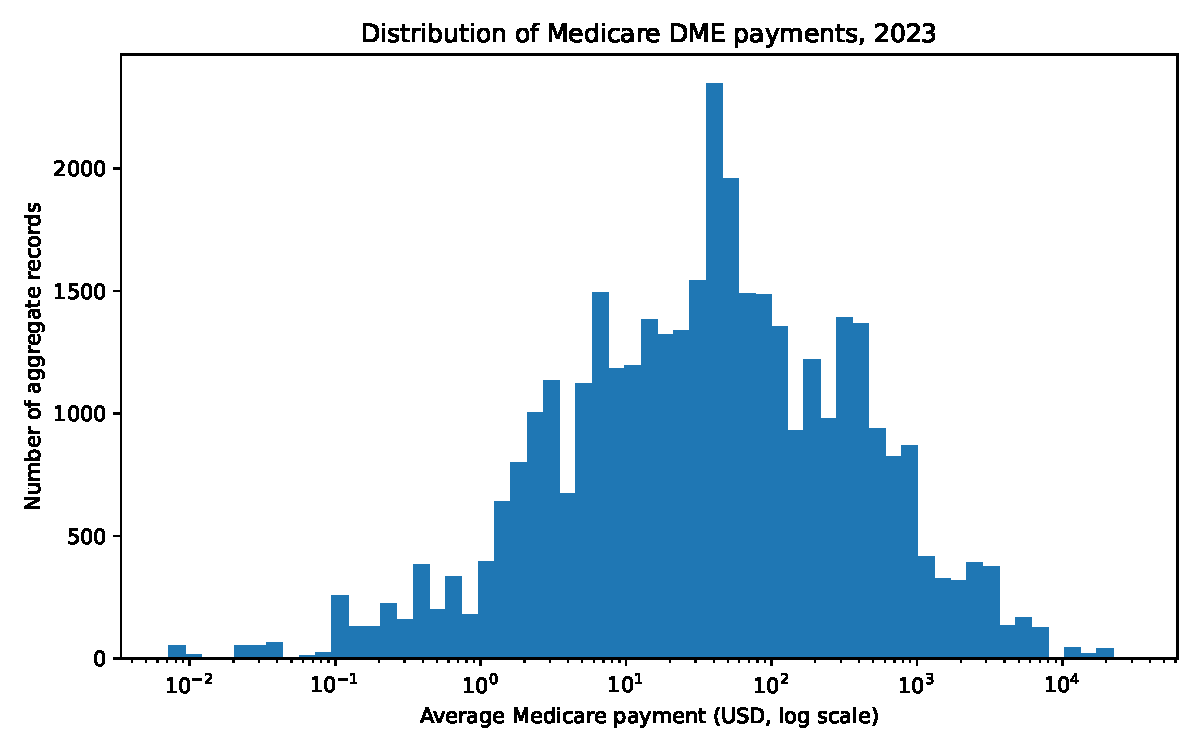
\includegraphics[width=.61\linewidth]{payment_distribution.pdf}
\caption{Observed average Medicare DME payments in the preliminary 60-category exploratory dataset, displayed on a logarithmic horizontal axis.}\label{fig:distribution}\end{figure}
\begin{figure}[!htbp]\centering
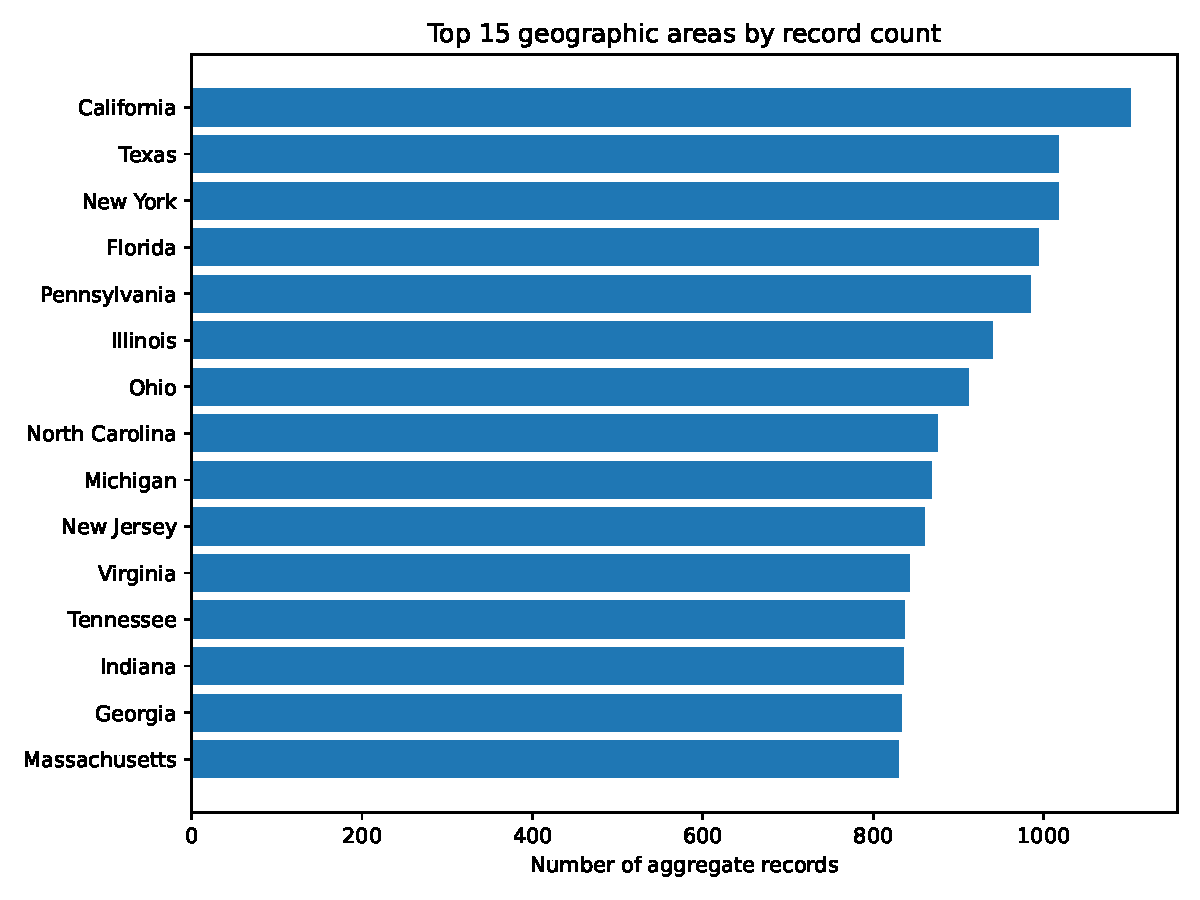
\includegraphics[width=.61\linewidth]{geographic_coverage.pdf}
\caption{Fifteen geographic categories with the greatest number of aggregate records in the exploratory dataset.}\label{fig:coverage}\end{figure}

\subsection{Preliminary Baselines and Geographic Holdout}
On the initial random 80/20 split of the 60-category dataset, the global-mean baseline had an MAE of \$458.62 and an RMSE of \$1,210.88. The HCPCS-mean baseline reduced these to \$48.97 and \$265.43. Across 30 preliminary split seeds, mean random-split HCPCS MAE was \$49.07 and mean geographic-holdout MAE was \$47.60. Geographic holdout produced larger MAE in 12 of 30 comparisons, so these experiments do not support a claim that random splitting invariably understates error.
\begin{table}[!htbp]\centering
\caption{Preliminary results on the 60-category population.}\label{tab:preliminary}
\begin{tabular}{lrr}\toprule
Random-split model & MAE (USD) & RMSE (USD)\\\midrule
Global training mean & 458.62 & 1210.88\\
HCPCS training mean & 48.97 & 265.43\\
\bottomrule\end{tabular}\end{table}
\subsection{Geographic Reliability and HCPCS Coverage}
For 51-area leave-one-area-out evaluation, the HCPCS-only baseline achieved an actual-payment micro MAE of \$47.84 and macro area MAE of \$46.27. Texas had the largest observed area MAE, \$103.55. The 36,391 test records with codes observed in training had MAE \$45.21. Only 137 records (0.38\%) had unseen HCPCS codes, but these had MAE \$747.00 and contributed 5.86\% of total absolute prediction error (Table~\ref{tab:coverage}).
\begin{table}[!htbp]\centering
\caption{Known versus unseen HCPCS code errors, 51-area HCPCS-only baseline.}\label{tab:coverage}
\begin{tabular}{lrrr}\toprule
Code status & Records & MAE (USD) & Error share\\\midrule
Known & 36,391 & 45.21 & 94.14\%\\
Unseen & 137 & 747.00 & 5.86\%\\
\bottomrule\end{tabular}\end{table}

\subsection{Payment Standardization and Within-Group Variation}
Among the 916 HCPCS/rental groups present in at least ten areas, the mean observed-payment CV was 0.09059 and the corresponding mean standardized-payment CV was 0.04744. Standardized CV was smaller in 805 groups (87.9\%), larger in 95 groups, and equal in 16 groups (Table~\ref{tab:cv}). The distribution of paired coefficients is displayed in Figure~\ref{fig:cv}. Since standardization is designed partly to remove policy-based payment differences, this result is interpreted as a descriptive check rather than as a novel standardization method.
\begin{table}[!htbp]\centering
\caption{Actual versus standardized within-group geographic variation.}\label{tab:cv}
\begin{tabular}{lr}\toprule
Measure & Value\\\midrule
Eligible HCPCS/rental groups & 916\\
Mean observed-payment CV & 0.09059\\
Mean standardized-payment CV & 0.04744\\
Groups with lower standardized CV & 805\\
Groups with higher standardized CV & 95\\
Groups with equal CV & 16\\
\bottomrule\end{tabular}\end{table}
\begin{figure}[!htbp]\centering
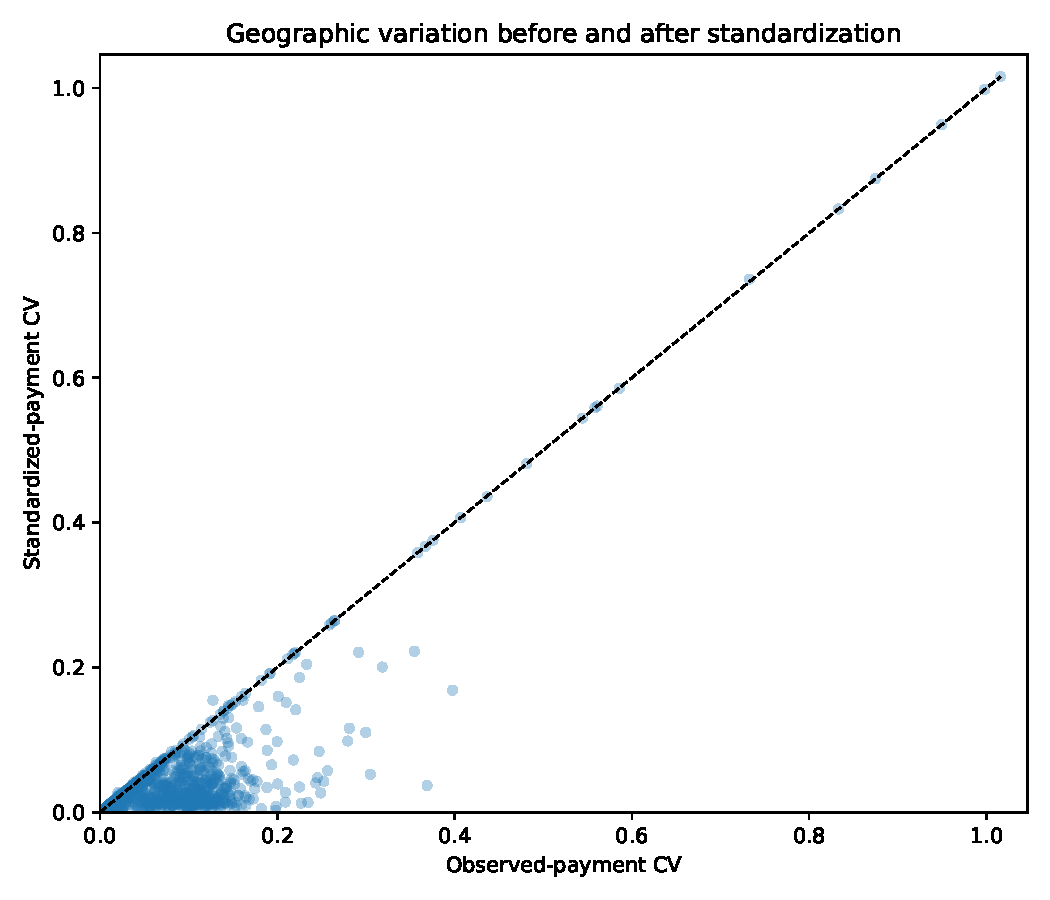
\includegraphics[width=.61\linewidth]{standardization_cv_comparison.pdf}
\caption{Observed and standardized coefficients of variation across 916 comparable HCPCS/rental groups. The dashed diagonal represents equal variation.}\label{fig:cv}\end{figure}

\subsection{Paired Target Prediction and Rental-Aware Analysis}
In paired leave-one-area-out testing, the HCPCS-only baseline had an actual-payment micro MAE of \$47.84, compared with \$38.88 for the standardized-payment target. The analogous RMSEs were \$290.78 and \$284.49. Both MAE and normalized MAE were smaller for the standardized target in every one of the 51 held-out geographic areas.

Including rental classification in the group-mean baseline reduced actual-payment MAE to \$19.89 and standardized-payment MAE to \$10.30, corresponding to reductions of 58.4\% and 73.5\% relative to the HCPCS-only baselines for the respective targets. Under the rental-aware specification, standardized-target MAE was lower in all 51 areas, while the worst-area MAEs were \$66.42 and \$54.63 for actual and standardized payments, respectively (Table~\ref{tab:models}). The improvements in RMSE were substantially smaller than those in MAE, indicating that large residual errors remain influential.
\begin{table}[!htbp]\centering\small
\caption{Leave-one-area-out prediction errors on the 51-area primary population. Each target is predicted separately.}\label{tab:models}
\begin{tabular}{llrrrr}\toprule
Model & Target & MAE & RMSE & NMAE\% & Worst MAE\\\midrule
HCPCS & Actual & 47.84 & 290.78 & 14.48 & 103.55\\
HCPCS & Standardized & 38.88 & 284.49 & 11.71 & 92.72\\
HCPCS+rental & Actual & 19.89 & 185.67 & 6.02 & 66.42\\
HCPCS+rental & Standardized & 10.30 & 182.01 & 3.10 & 54.63\\
\bottomrule\end{tabular}\end{table}


\FloatBarrier

% DISCUSSION
\section{Discussion}
\label{sec:discussion}
\subsection{Equipment Classification and Prediction Error}
The largest change in average absolute prediction error resulted from including the rental indicator alongside the HCPCS code. The actual-payment MAE decreased from \$47.84 to \$19.89 under the same 51-area holdout protocol. This suggests that averaging across rental statuses within a code discards predictive information relevant to the aggregate payments in this dataset. The improvement is attributable to a more specific descriptive baseline, not to a learned nonlinear representation. The code/rental grouping is also consistent with the unit of comparison used in the geographic coefficient-of-variation analysis.

\subsection{Standardized Targets Are Different Outcomes}
Standardized average payments had lower MAE and pooled NMAE than observed average payments for both baselines. Under rental-aware prediction, the two micro MAEs were \$10.30 and \$19.89. This direction was consistent across all 51 areas. The finding is compatible with the motivation for Medicare payment standardization described by O'Donnell et al.~\citep{odonnell2013}: some geographic payment variation is attributable to reimbursement adjustments rather than to the underlying service mix. Nevertheless, the two errors measure predictions of \emph{different target fields}. A smaller error for standardized payments does not establish that predicting the actual Medicare payment has improved. We did not evaluate a procedure that predicts standardized amounts and then transforms them back into observed payments.

\subsection{Uneven Geographic Reliability}
Pooled accuracy obscures geographic heterogeneity. For example, under the HCPCS-only actual-payment baseline, the macro MAE was \$46.27 while the highest area MAE was \$103.55 in Texas. The latter value cannot be interpreted as evidence of an intrinsic disadvantage associated with Texas: differences in HCPCS composition, rental mix, and availability of codes across training areas may contribute. The preliminary 30-seed comparison also did not show geographically grouped holdout consistently exceeding random-split error, emphasizing the need to examine both the evaluation design and test-set composition \citep{roberts2017}.

\subsection{Rare Codes and Residual Errors}
Unseen HCPCS codes comprised approximately 0.38\% of held-out observations under the HCPCS-only baseline but generated about 5.86\% of its total absolute error. The fallback to a global mean can be far from the appropriate amount for an unusual code. This is a useful diagnostic for model deployment because average accuracy may conceal occasional large errors. We have not established whether the worst errors arise from rare equipment types, claim aggregation, geographic payment adjustment, or other factors; such explanations require additional analysis.

\subsection{Limitations and Future Work}
The study uses one year of publicly released aggregate CMS records, which can reflect disclosure suppression and differences in service volume \citep{cmsdme2023}. The measured MAE is an unweighted average across aggregated rows; it does not represent beneficiary-level error or total expenditure error. The same payment-code hierarchy was used across targets, but target magnitudes and distributions are not identical, so percentage error reductions should not be interpreted as causal estimates of standardization's effect. In addition, no independent future-year test, statistical uncertainty interval for geographic comparisons, or flexible machine-learning model benchmark was completed. Dataset shift across time or settings remains a concern \citep{subbaswamy2020}. Future work could repeat the analysis across years, use service-volume-weighted metrics alongside unweighted metrics, evaluate within-code residual geography effects, and compare transparent baselines with more flexible estimators using equivalent geographic splits.

% CONCLUSION
\section{Conclusion}
\label{sec:conclusion}
Using 36,528 aggregated 2023 Medicare DME records from the 50 U.S. states and Washington, DC, this study evaluated geographic prediction reliability using interpretable group-mean baselines. Distinguishing HCPCS codes by rental classification reduced actual-payment leave-one-area-out MAE from \$47.84 to \$19.89. Standardized average payments were also easier to predict under the tested baselines, with rental-aware MAE of \$10.30, and their area-level MAE was lower in all 51 held-out areas. Rare unseen HCPCS codes nonetheless accounted for a disproportionate share of absolute error under the HCPCS-only baseline. These findings demonstrate why payment-target definitions, equipment classification, code coverage, and area-specific errors should accompany pooled accuracy when evaluating geographic reliability. They do not establish causality or a universally superior prediction model; validation on additional years and modeling approaches is necessary.


% ============================================
% MANUAL REFERENCES
% ============================================

% references_manual.tex contains the
% thebibliography environment and 10 entries.
% Do not run BibTeX for this document.

% Numeric bibliography: works with natbib [numbers], no BibTeX required.
\begin{thebibliography}{10}
\bibitem{cmsdme2023}
Centers for Medicare \& Medicaid Services (CMS). \emph{Medicare Durable Medical Equipment, Devices \& Supplies --- by Geography and Service}, 2023 data year. \url{https://data.cms.gov/provider-summary-by-type-of-service/medicare-durable-medical-equipment-devices-supplies/medicare-durable-medical-equipment-devices-supplies-by-geography-and-service}.

\bibitem{roberts2017}
Roberts, D. R., Bahn, V., Ciuti, S., et al. Cross-validation strategies for data with temporal, spatial, hierarchical, or phylogenetic structure. \emph{Ecography}, 40(8):913--929, 2017. \url{https://doi.org/10.1111/ecog.02881}.

\bibitem{odonnell2013}
O'Donnell, B. E., Schneider, K. M., Brooks, J. M., et al. Standardizing Medicare payment information to support examining geographic variation in costs. \emph{Medicare \& Medicaid Research Review}, 3(3), 2013. \url{https://doi.org/10.5600/mmrr.003.03.a06}.

\bibitem{subbaswamy2020}
Subbaswamy, A. and Saria, S. From development to deployment: dataset shift, causality, and shift-stable models in health AI. \emph{Biostatistics}, 21(2):345--352, 2020. \url{https://doi.org/10.1093/biostatistics/kxz041}.

\bibitem{pedregosa2011}
Pedregosa, F., Varoquaux, G., Gramfort, A., et al. Scikit-learn: Machine learning in Python. \emph{Journal of Machine Learning Research}, 12:2825--2830, 2011. \url{https://www.jmlr.org/papers/v12/pedregosa11a.html}.

\bibitem{kohavi1995}
Kohavi, R. A study of cross-validation and bootstrap for accuracy estimation and model selection. In \emph{Proceedings of the 14th International Joint Conference on Artificial Intelligence}, pp. 1137--1145, 1995. \url{https://mlanthology.org/ijcai/1995/kohavi1995ijcai-study/}.

\bibitem{steyerberg2010}
Steyerberg, E. W., Vickers, A. J., Cook, N. R., et al. Assessing the performance of prediction models: a framework for traditional and novel measures. \emph{Epidemiology}, 21(1):128--138, 2010. \url{https://doi.org/10.1097/EDE.0b013e3181c30fb2}.

\bibitem{arlot2010}
Arlot, S. and Celisse, A. A survey of cross-validation procedures for model selection. \emph{Statistics Surveys}, 4:40--79, 2010. \url{https://doi.org/10.1214/09-SS054}.

\bibitem{cawley2010}
Cawley, G. C. and Talbot, N. L. C. On over-fitting in model selection and subsequent selection bias in performance evaluation. \emph{Journal of Machine Learning Research}, 11:2079--2107, 2010. \url{https://www.jmlr.org/papers/v11/cawley10a.html}.

\bibitem{varma2006}
Varma, S. and Simon, R. Bias in error estimation when using cross-validation for model selection. \emph{BMC Bioinformatics}, 7:91, 2006. \url{https://doi.org/10.1186/1471-2105-7-91}.

\end{thebibliography}


\end{document}
